\documentclass[12pt,a4paper]{report}
\usepackage[italian]{babel}
\usepackage[T1]{fontenc}
\usepackage{geometry}
\usepackage{graphicx}
\usepackage{hyperref}
\usepackage[utf8]{inputenc}
\usepackage{subcaption}
\usepackage[nottoc,numbib]{tocbibind}
\usepackage{titlesec}
\titleformat{\chapter}[display]{\Huge\bfseries}{}{0pt}{\thechapter.\ }
\graphicspath{{figures/}}
\begin{document}

\newgeometry{margin=1in}
\begin{titlepage}
	\centering
	
\includegraphics[width=0.34\textwidth]{logo-unipg}\par\vspace{1cm}
	\large{Tesina Finale di}\par
	\large{\textbf{Programmazione Interfacce Grafiche e Dispositivi Mobili}}\par
	\small{Corso di Laurea in Ingegneria Informatica ed Elettronica -- A.A. 2023-2024}\par
	\textsc{\small{Dipartimento di Ingegneria}}\par
	%\large{A.A. 2023-2024}\par

	%\vfill
	\vspace{0.5cm}
	docente\par
	Prof. Luca \textsc{Grilli}

	\vspace{1cm}
	\vspace{1cm}
	\textbf{\huge{ClickMania}}\par
	\vspace{0.2cm}
	gioco di sopravvivenza a livelli\par
	\vspace{0.5cm}
	
\includegraphics[width=0.50\textwidth]{LaTeX-template-PIGDM/figures/logo_game.png}\par\vspace{1cm}
	\vspace{1cm}

	\begin{tabular}{ l l l l }
	\large{344955} & \large{\textbf{Aiman}} & \large{\textbf{Rattab}} & \large{aiman.rattab@studenti.unipg.it}\\
	\end{tabular}

	\vfill
	\raggedright
	\small{Data ultimo aggiornamento: \today}
\end{titlepage}

\restoregeometry
\tableofcontents

\chapter{Descrizione del Problema}\label{ch:despro}

Questo progetto ha come obiettivo lo sviluppo di un videogioco desktop  ispirato al genere \emph{roguelike-lite} e
in particolare al successo di "Vampire Survivors". Partendo dalle meccaniche di base del genere, ovvero la sopravvivenza in
un'arena invasa da nemici, si propone un'esperienza di gioco arricchita da elementi originali. L'introduzione di lanciagranate,
pistole, e di un sistema di ostacoli dinamici, come percorsi di lava e laghi e fiumi, contribuisce a creare un gameplay piu' strategico,
che lascia inoltre la possibilita' di arricchirlo in futuro con sempre piu' ostacoli e nuove meccaniche di combattimento.

\medskip
L'applicazione, sviluppata utilizzando la tecnologia JFC/Swing, garantisce una portabilità ottimale su diverse piattaforme,
permettendo a un vasto pubblico di godere di questo gioco di sopravvivenza.
\begin{figure}[h]
    \centering
    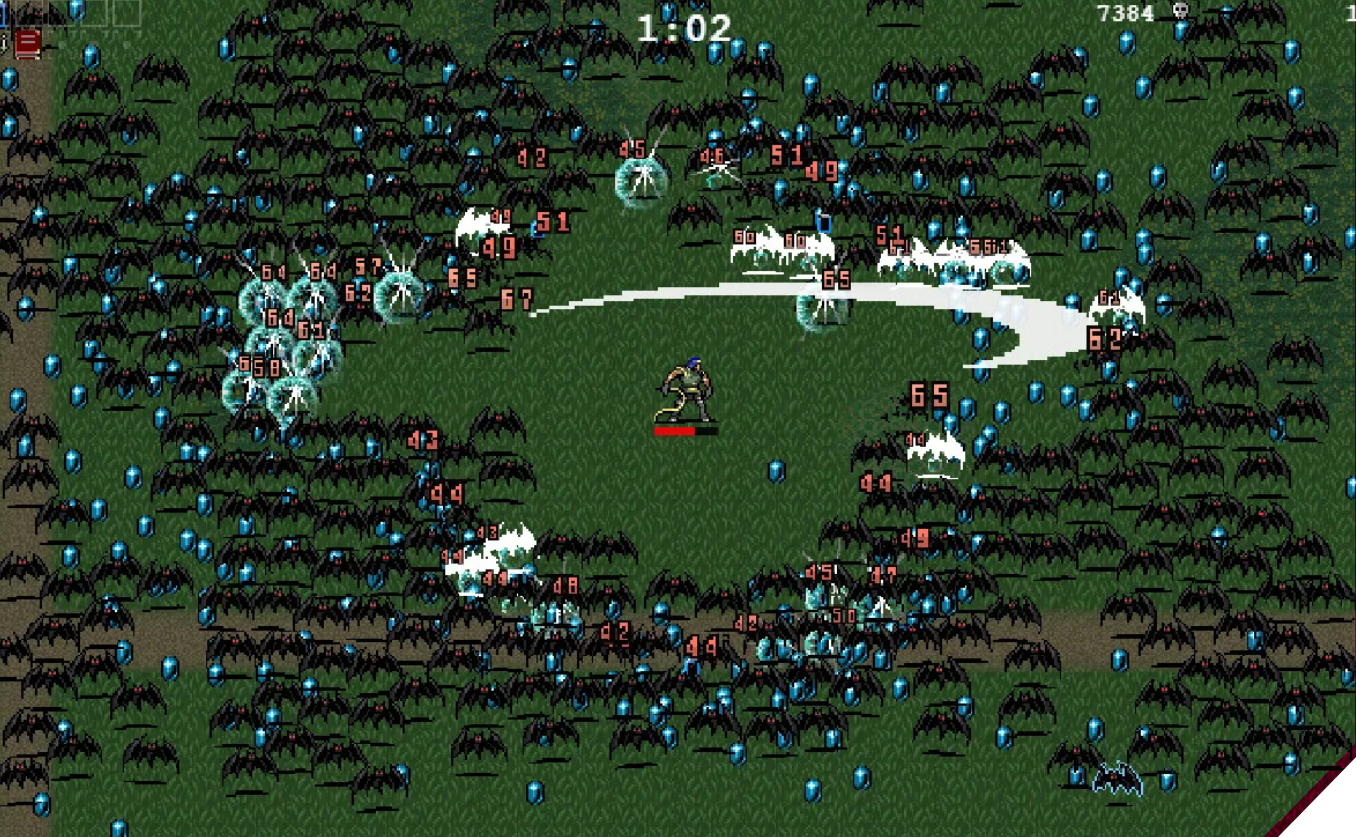
\includegraphics[width=0.8\textwidth]{vs}
    \caption{Esempio di Gameplay di Vampire-survivors}
    \label{fig:enter-label}
\end{figure}

\newpage
\chapter{L'applicazione Click Mania}\label{se:appjgal}
L'azione è al centro del gameplay. Il protagonista, visto dall'alto, si muove in un'arena caotica, circondato da orde di nemici.
La fluidità dei movimenti, sia del personaggio che degli avversari, crea un'esperienza di gioco dinamica e coinvolgente.
L'obiettivo è semplice: eliminare tutti i nemici presenti sullo schermo prima che raggiungano il giocatore.
Tuttavia, la sfida aumenta progressivamente visto l'aumento del numero di nemici con l'avanzare dei livelli.\\
\begin{figure}[h]
    \centering
    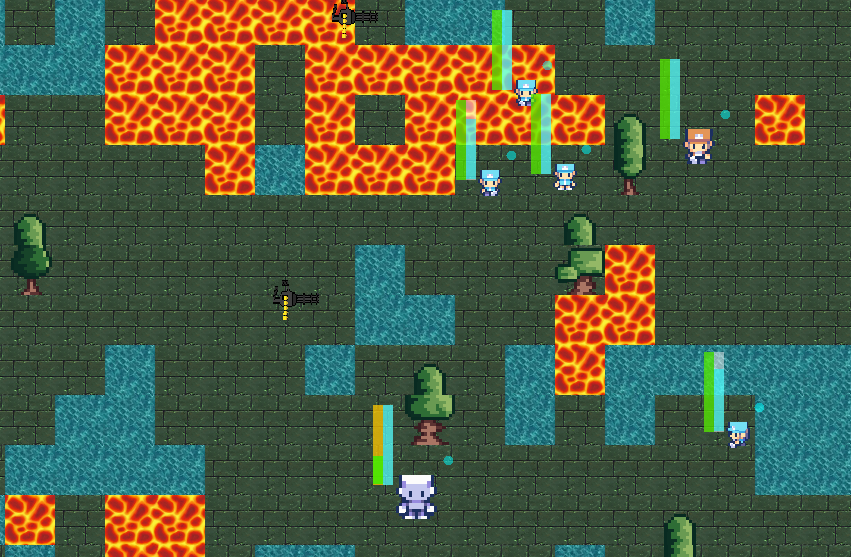
\includegraphics[width=1\textwidth]{cmgp}
    \caption{Esempio di Gameplay di Vampire-survivors}
    \label{fig:enter-label}
\end{figure}

\newpage
\section{Specifica dei requisiti}\label{se:appjgal}
L’applicazione Clickmania che intendo realizzare dovrà soddisfare i seguenti requisiti:
\begin{itemize}
\item Presenza di una fisica di movimento realistica (incluso attrito)
\item Presenza di alberi che bloccano il passaggio
\item Presenza di acqua che riduce la velocita'
\item Presenza di un knockback causato dai proiettili.
\item Possibilita' di raccogliere fino a 10 armi in giro per la mappa
\item Possibilita' di mettere in pausa il gioco
\item Presenza di punti di spawn per nemici (i nemici dovranno girare solo nel loro punto di spawn, a meno che non inseguino il giocatore)
\item Presenza di un' area di visione delle entita' (se il giocatore entra in questa area, il nemico si accorge di lui e lo insegue)
\item repulsione dei vari nemici tra di loro (evitando accumuli di nemici)
\item tempo di ricarica delle armi (sia giocatore che nemici)
\item Possibilita' di scambiare un arma con un'altra nell'inventario tramite tastierino numerico
\item scalare la finestra a proprio piacimento
\item possibilita' di  personalizzare tutti i parametri dei vari nemici e il giocatore tramite files json
\item avere una creazione della mappa procedurale, tramite seed
\item Presenza di livelli illimitati
\item Animazione skin personaggi in movimento
\item Presenza di acqua che aumenta l'attrito
\item Presenza di lava che aumenta attrito e provoca danno al player
\item Presenza di barra per la salute visibile
\end{itemize}
\newpage

\chapter{Progetto}\label{ch:spereq}

Il progetto è stato strutturato in modo da favorire la modularità e la riutilizzabilità del codice.
Attraverso la creazione di classi specializzate per gestire le diverse componenti del gioco (come entità, armi, mappe),
è stato possibile organizzare il codice in modo più chiaro e facilitare l'aggiunta di nuove funzionalità.
Questa scelta progettuale ha permesso di ridurre la duplicazione del codice e di rendere il gioco più facilmente espandibile.
\begin{figure}[h]
    \centering
    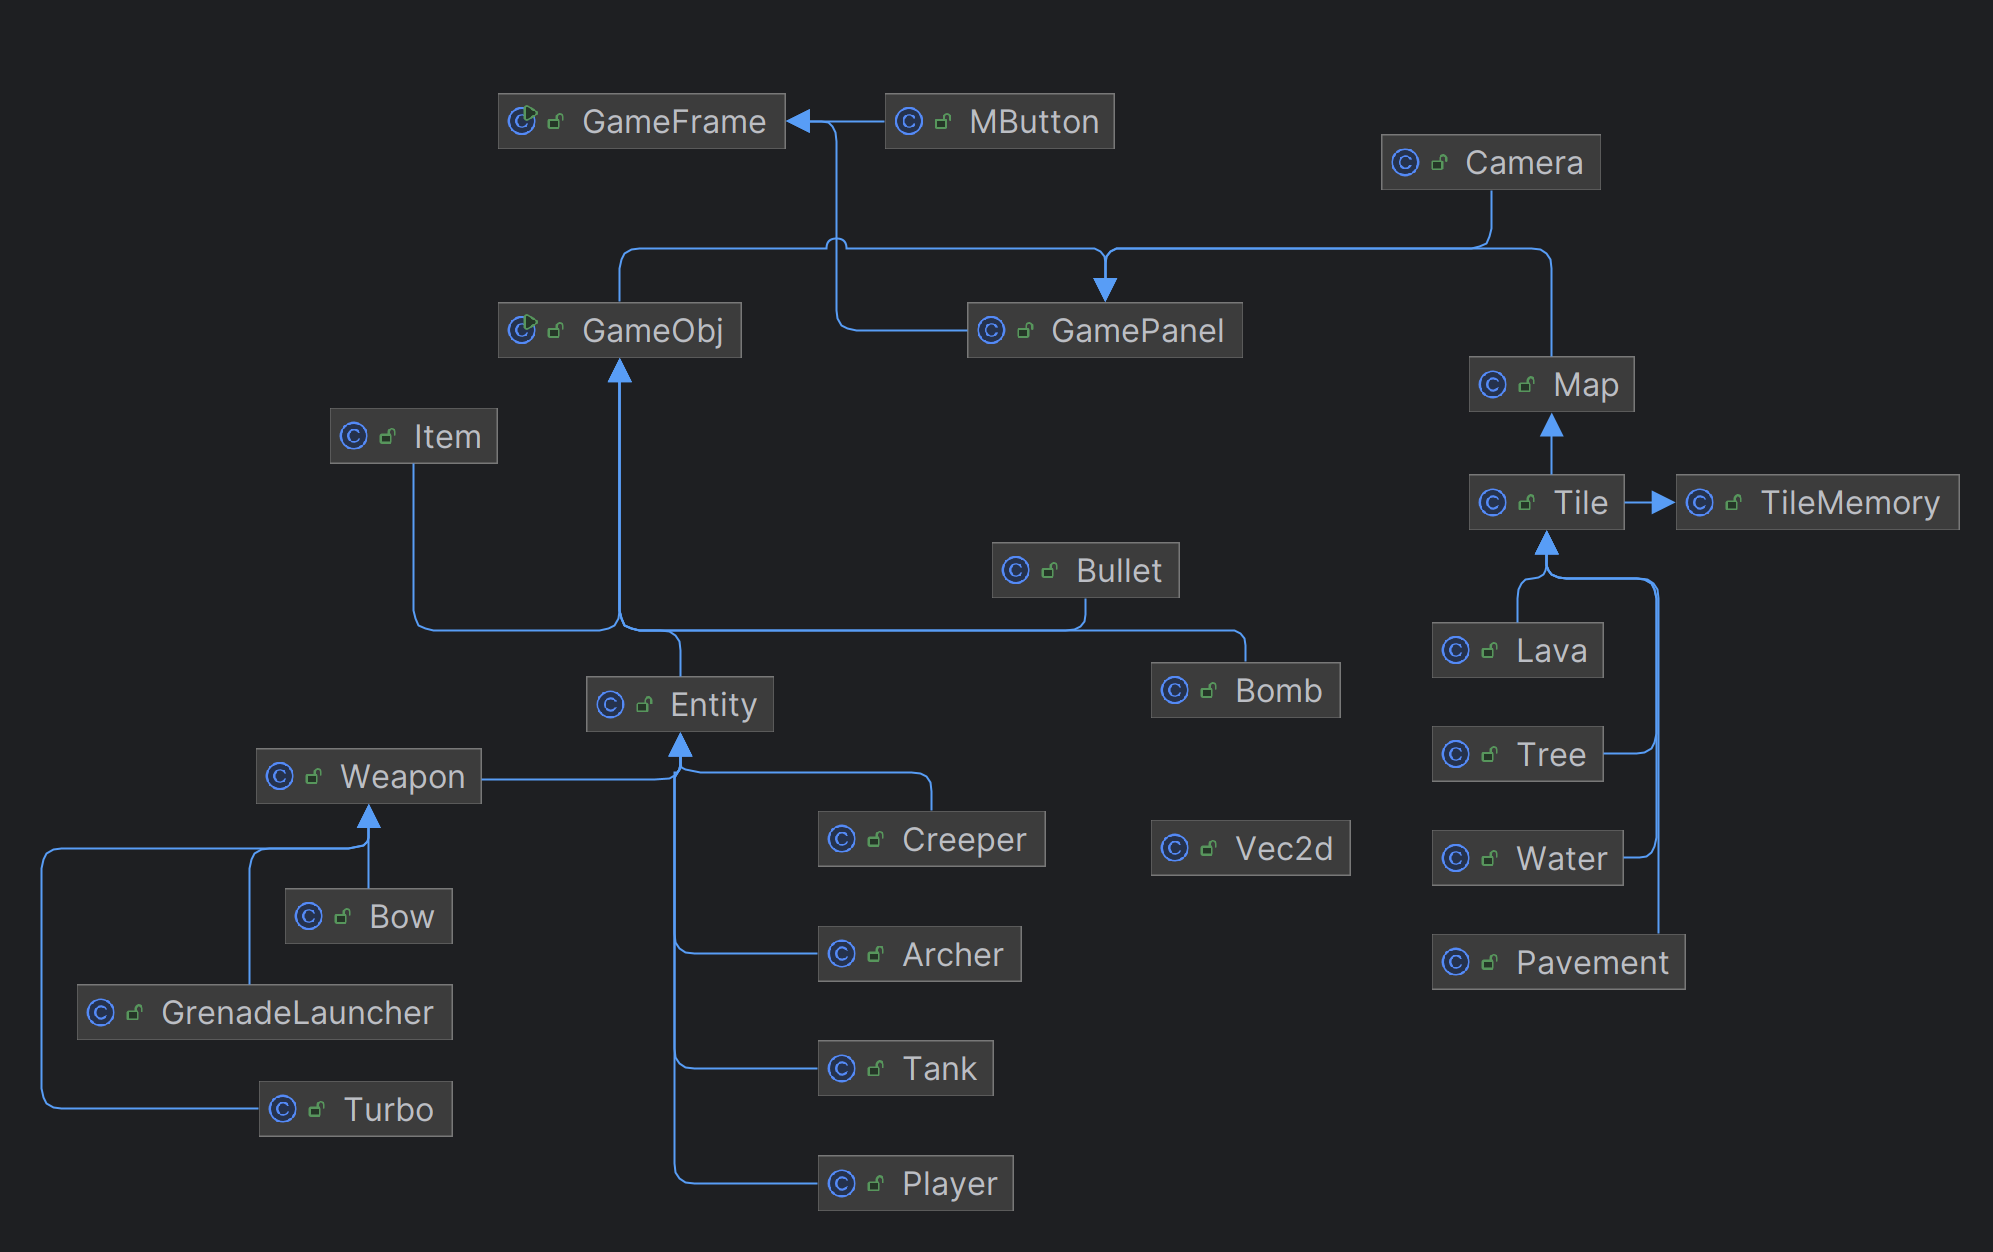
\includegraphics[width=1\textwidth]{LaTeX-template-PIGDM/figures/uml_clickmania.png}
    \caption{Architettura con interazioni tra classi di tutti i pacchetti}
    \label{fig:enter-label}
\end{figure}
\\

\section{Architettura del sistema software}\label{se:appjgal}


non ho voluto seguire la struttura model view controller poiche' ho pensato che raggruppare i vari oggetti del gioco in weapons,
entities, map e gamelogic sia piu' ordinato; specialmente se si prevede di ampliare il gioco con piu' entita' e armi.
L'architettura del gioco è basata su una gerarchia di classi ben definita. La classe base GameObj rappresenta qualsiasi oggetto nel
gioco e fornisce metodi virtuali per l'aggiornamento e il rendering degli oggetti, e la gestione delle collisioni.
Le classi Entity, Bomb, Item e Bullet ereditano da GameObj e implementano comportamenti specifici. Il GamePanel è responsabile
del ciclo di gioco, dell'aggiornamento di tutte le entità e del rendering della scena. La mappa è rappresentata da una matrice di
tipo GameObj, e contiene informazioni sugli ostacoli e sul terreno (vi sono 2 distinte matrici per suddividere tra entita' e tipo
di terreno). Per ottimizzare le prestazioni, il rendering è limitato agli oggetti visibili sullo schermo e viene utilizzata una
struttura dati spaziale per accelerare le query di collisione.
Il GameFrame è il cuore del gioco, gestendo sia la logica di gioco che l'interfaccia utente. Gli eventi generati dall'interfaccia utente,
come i clic sui pulsanti del menu, vengono intercettati dal GameFrame, che aggiorna di conseguenza lo stato del gioco.
Ad esempio, quando l'utente clicca sul pulsante "play", il GameFrame nasconde il JPanel del menu, resetta il gioco,
riavvia il timer e riinizia il gameplay. Questa architettura modulare permette di separare la logica di gioco dall'interfaccia utente,
facilitando la manutenzione e l'espansione del gioco.\\
nel metodo paintComponent() (richiamato ad ogni frame per disegnare su schermo tutti gli oggetti visibili), all'interno del JPanel,
ho preferito suddividere la logica in 2, disegnando prima il background del gioco (pavimento, acqua, lava e alberi),
e poi sopra di essi le skin delle varie entita' (poiche' sono piu' piccole e non avrebbe avuto senso fare il contrario).
\\\\
\newpage
\section{Descrizione dei moduli}\label{se:appjgal}
\begin{figure}[h]
    \centering
    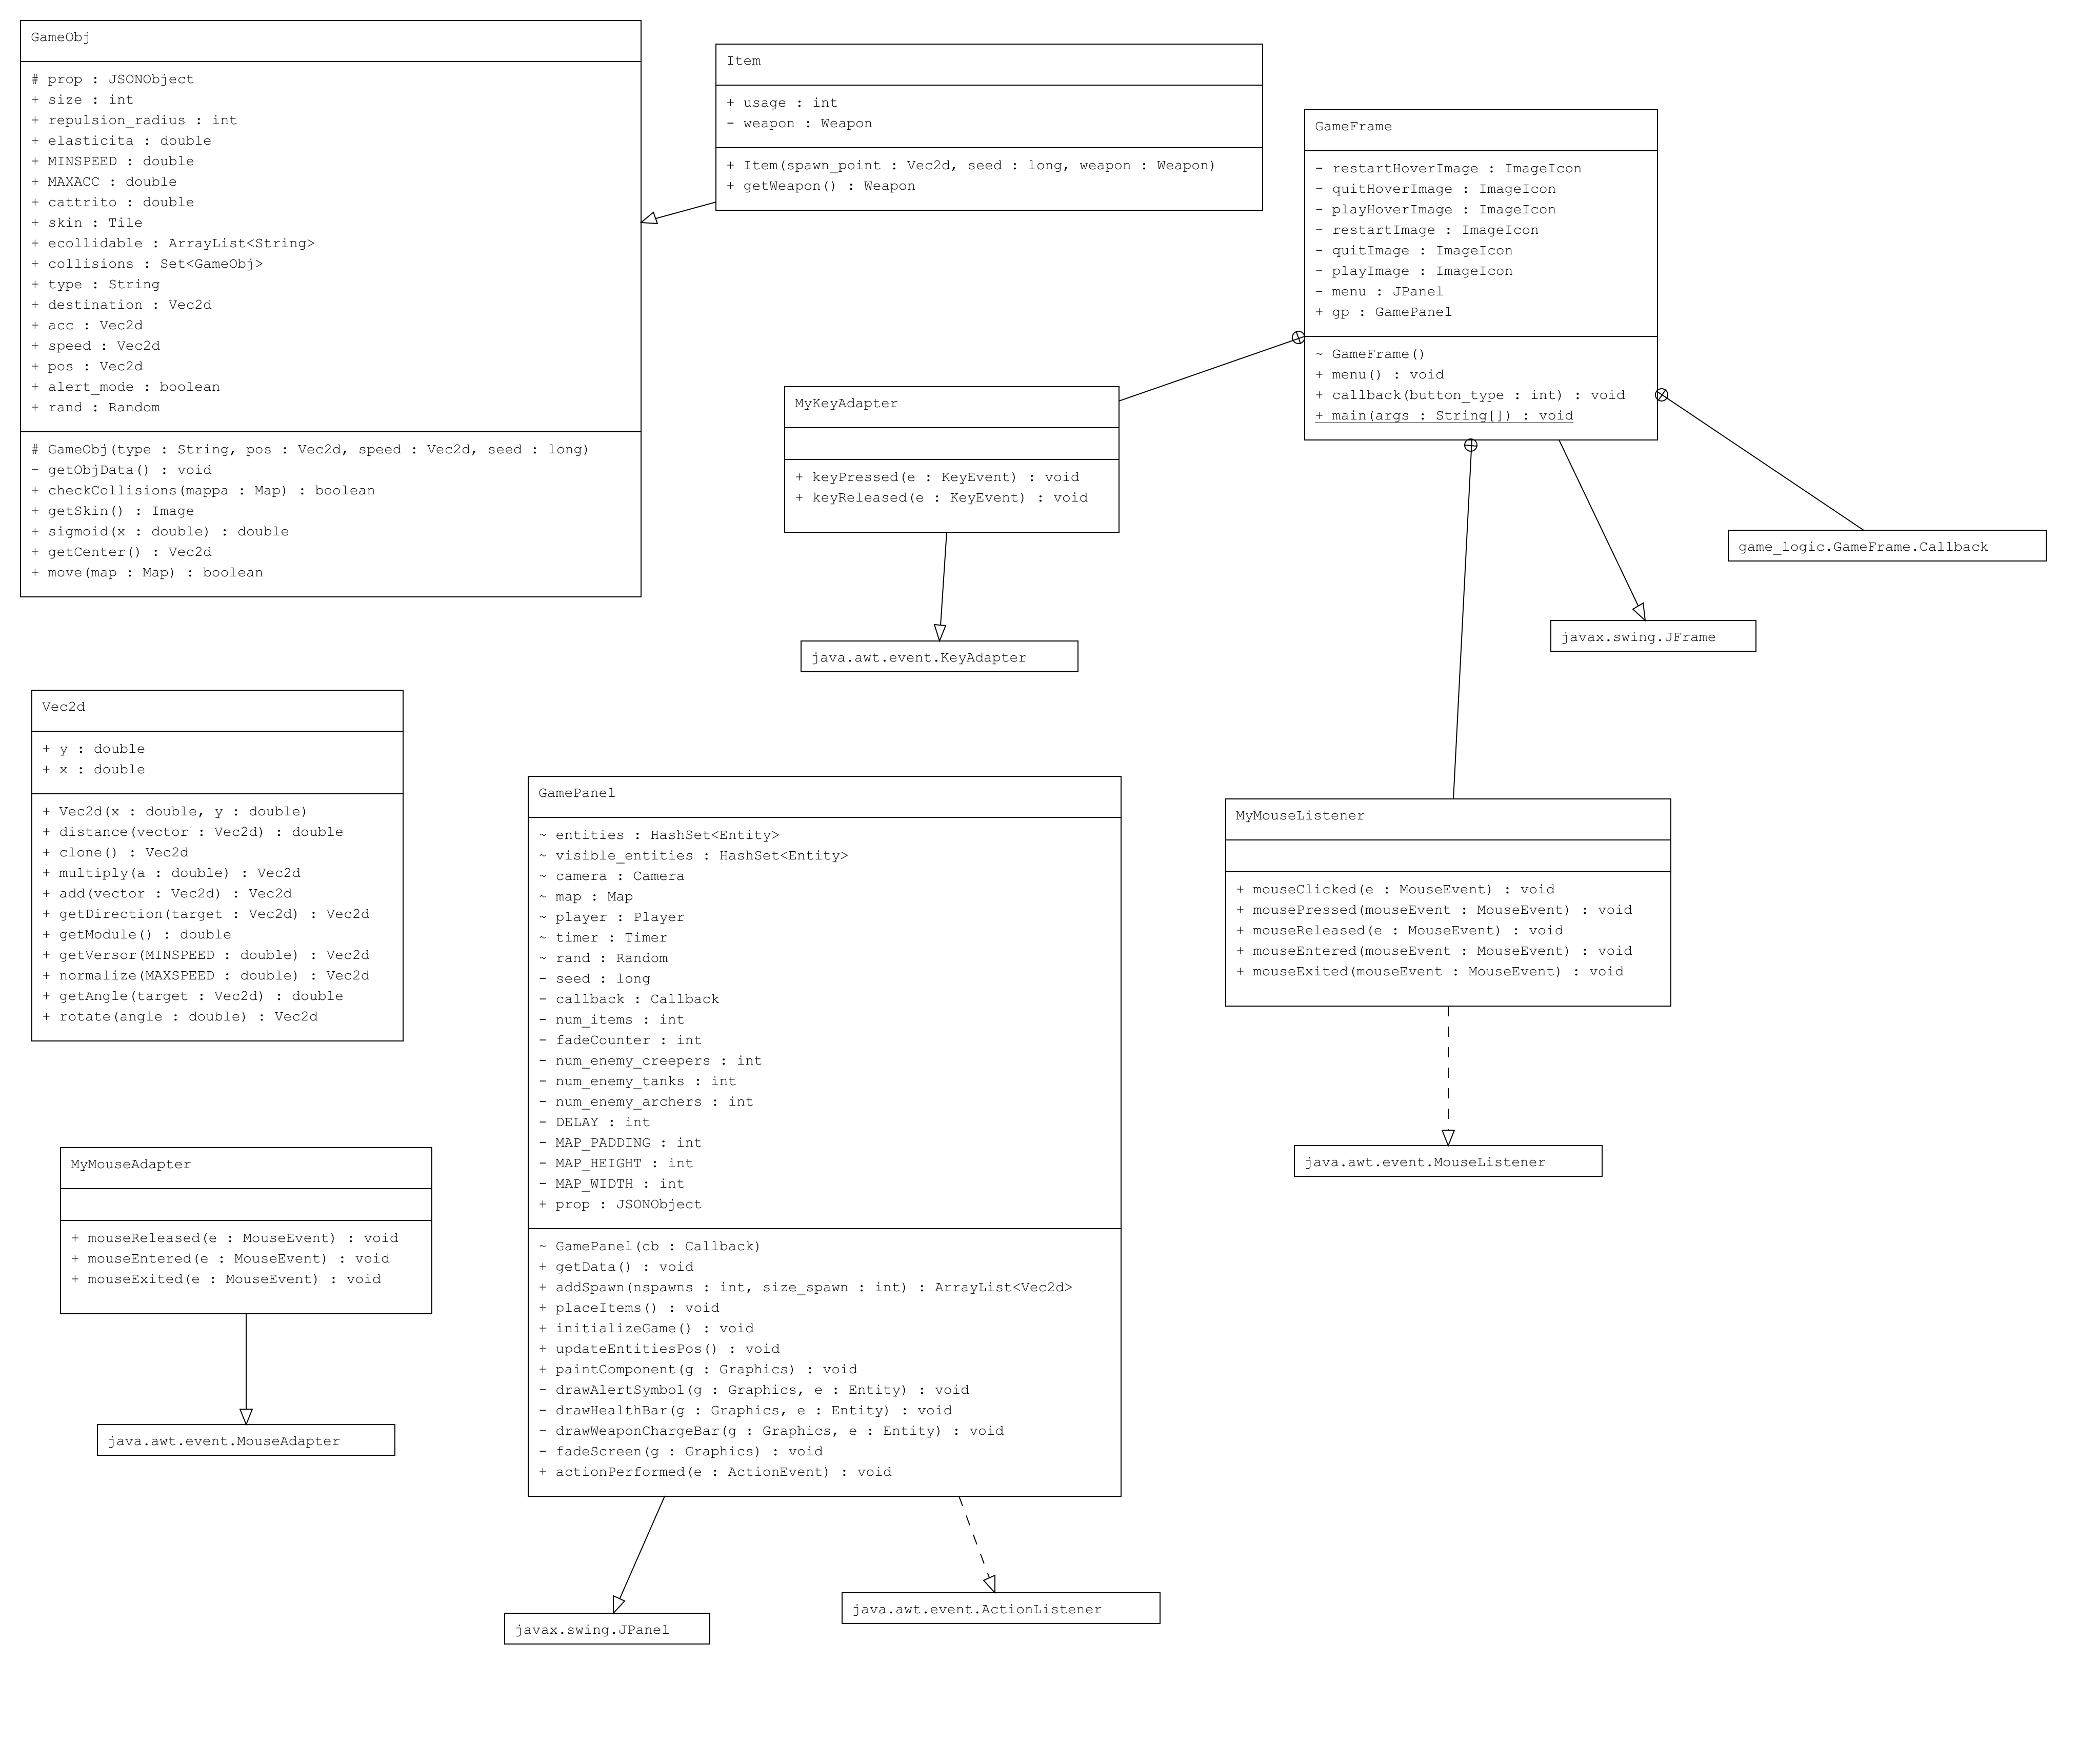
\includegraphics[width=1.1\textwidth]{LaTeX-template-PIGDM/figures/game_logic.png}
    \caption{diagramma uml delle varie classi all'interno di game\_logic}
    \label{fig:enter-label}
\end{figure}
all'interno del pacchetto game\_logic, vi ho inserito tutte le classi indispensabili per la logica e funzionamento del gioco.
Vediamo nel dettagli le classi piu' importanti:


\begin{itemize}
\item GameObj: la classe principale che verra' ereditata da tutti gli "oggetti" fisici del gioco; sono presenti i seguenti attributi
(i quali vengono dinamicamente letti dal file json dell'oggetto da instanziare):
\begin{itemize}
\item prop : la variabile di tipo JSONObject (ovvero un dizionario) che andra' a contenere tutti i dati dell' oggetto da istanziare (nel dizionario tutti i paramentri sono salvati come stringa, quindi vanno ancora castati al tipo giusto)
\item size: dimensioni oggetto
\item repulsion\_radius: un numero che indica quanto un oggetto sia repellente (si puo' anche immaginare come la quantita' di "carica positiva" che ha un oggetto, prorpio come si repellono elettroni tra loro)
\item elasticita: numero che indica quanto un oggetto rimbalza se collide
\item cattrito: coefficiente di attrito (ho deciso di metterlo sia negli oggetti che nel tipo di pavimentazione)
\item skin: la skin dell'oggetto, di tipo Tile (vedi piu' avanti)
\item ecollidable: un array che contiene i tipi di entita' con i quali questo puo' entrare in collisione (per rendere gioco piu' veloce, almeno inizialmente, rimuovevo le collisioni per entita' di tipo diverso)
\item collisions: contiene la lista di oggetti con le quali ha appena colliso (nel frame precedente)
\item type: tipo di oggetto
\item destination: destinazione (se ce l'ha) dell'oggetto
\item alert\_mode: (solo per nemici) indica se un entita' si e' accorta o meno della presenza del giocatore
\end{itemize}
i metodi di GameObj, invece, sono:
\begin{itemize}
\item checkCollisions(mappa): controlla le collisioni dell' oggetto con pareti o alberi
\item getSkin(): restituisce la sprite corretta dell'oggetto
\item getCenter(): restituisce il centro dell'oggetto (la posizione)
\item move(mappa): aggiorna posizione dell'oggetto.
\end{itemize}

\item GamePanel : questa classe sara' il canvas dove avvengono tutte le proiezioni a schermo dei vari oggetti e personaggi; inoltre si occupa di richiamare ad ogni frame i metodi degli oggetti per aggiornare la loro posizione. Gli attributi principali sono:
\begin{itemize}
\item entities: un Set di entita' che contiene tutte le entita' presenti nella mappa
\item visible\_entities: un Set contenente solo le entita' visibili su schermo
\item prop: JSONObject contenente tutte le impostazioni del gioco principale (come numero di nemici, dimensioni mappa ecc)
\end{itemize}
Adesso andiamo a vedere metodi principali del GamePanel:
\begin{itemize}
\item addSpawn(): restituisce una lista di spawnpoint random che non escono dalla mappa

\item placeItems(): inserisce nella mappa gli item (ovvero le armi raccoglibili dal giocatore) in maniera randomica

\item fadeScreen(): richiamata una volta che il giocatore muore, si tratta di una piccola animazione di fade.
\end{itemize}

\item Gameframe : questa classe fa da Frame a tutto il gioco, e gestisce sia gli input da tastiera che il menu di gioco.
i metodi sono i seguenti:
\begin{itemize}
\item menu(): crea e inserisce nel frame il menu di gioco con 3 pulsanti
\item callback(): metodo callback usato sia dal GamePanel che dai pulsanti (nella classe MButton) per gestire lo switch tra menu e gioco, e l'azzeramento dei livelli.
\item main(): metodo principale che fa partire il gioco.
\end{itemize}
Nel GameFrame ho aggiunto sia un mouseListener che un KeyAdapter. Partiamo con il descrivere i metodi del Keyadapter:
\begin{itemize}
\item keypressed(): gestisce i vari input di tastiera (w-a-s-d vanno a modificare l'accelerazione del giocatore in maniera opportuna, m e' usato per richiamare il menu, 1-2-3-4-5-6-7-8-9-0 sono usati per cambiare arma dall'inventario)
\item keyreleased(): rimuove accelerazione ad una direzione, in base al tasto rilasciato (w-a-s-d)
\end{itemize}
I metodi del MouseListener, invece, sono i seguenti:
\begin{itemize}
\item mouseReleased(): se il mouse viene rilasciato, faccio sparare al giocatore (se ne ha la possibilita')
\end{itemize}
\end{itemize}
\newpage

\begin{figure}[h]
    \centering
    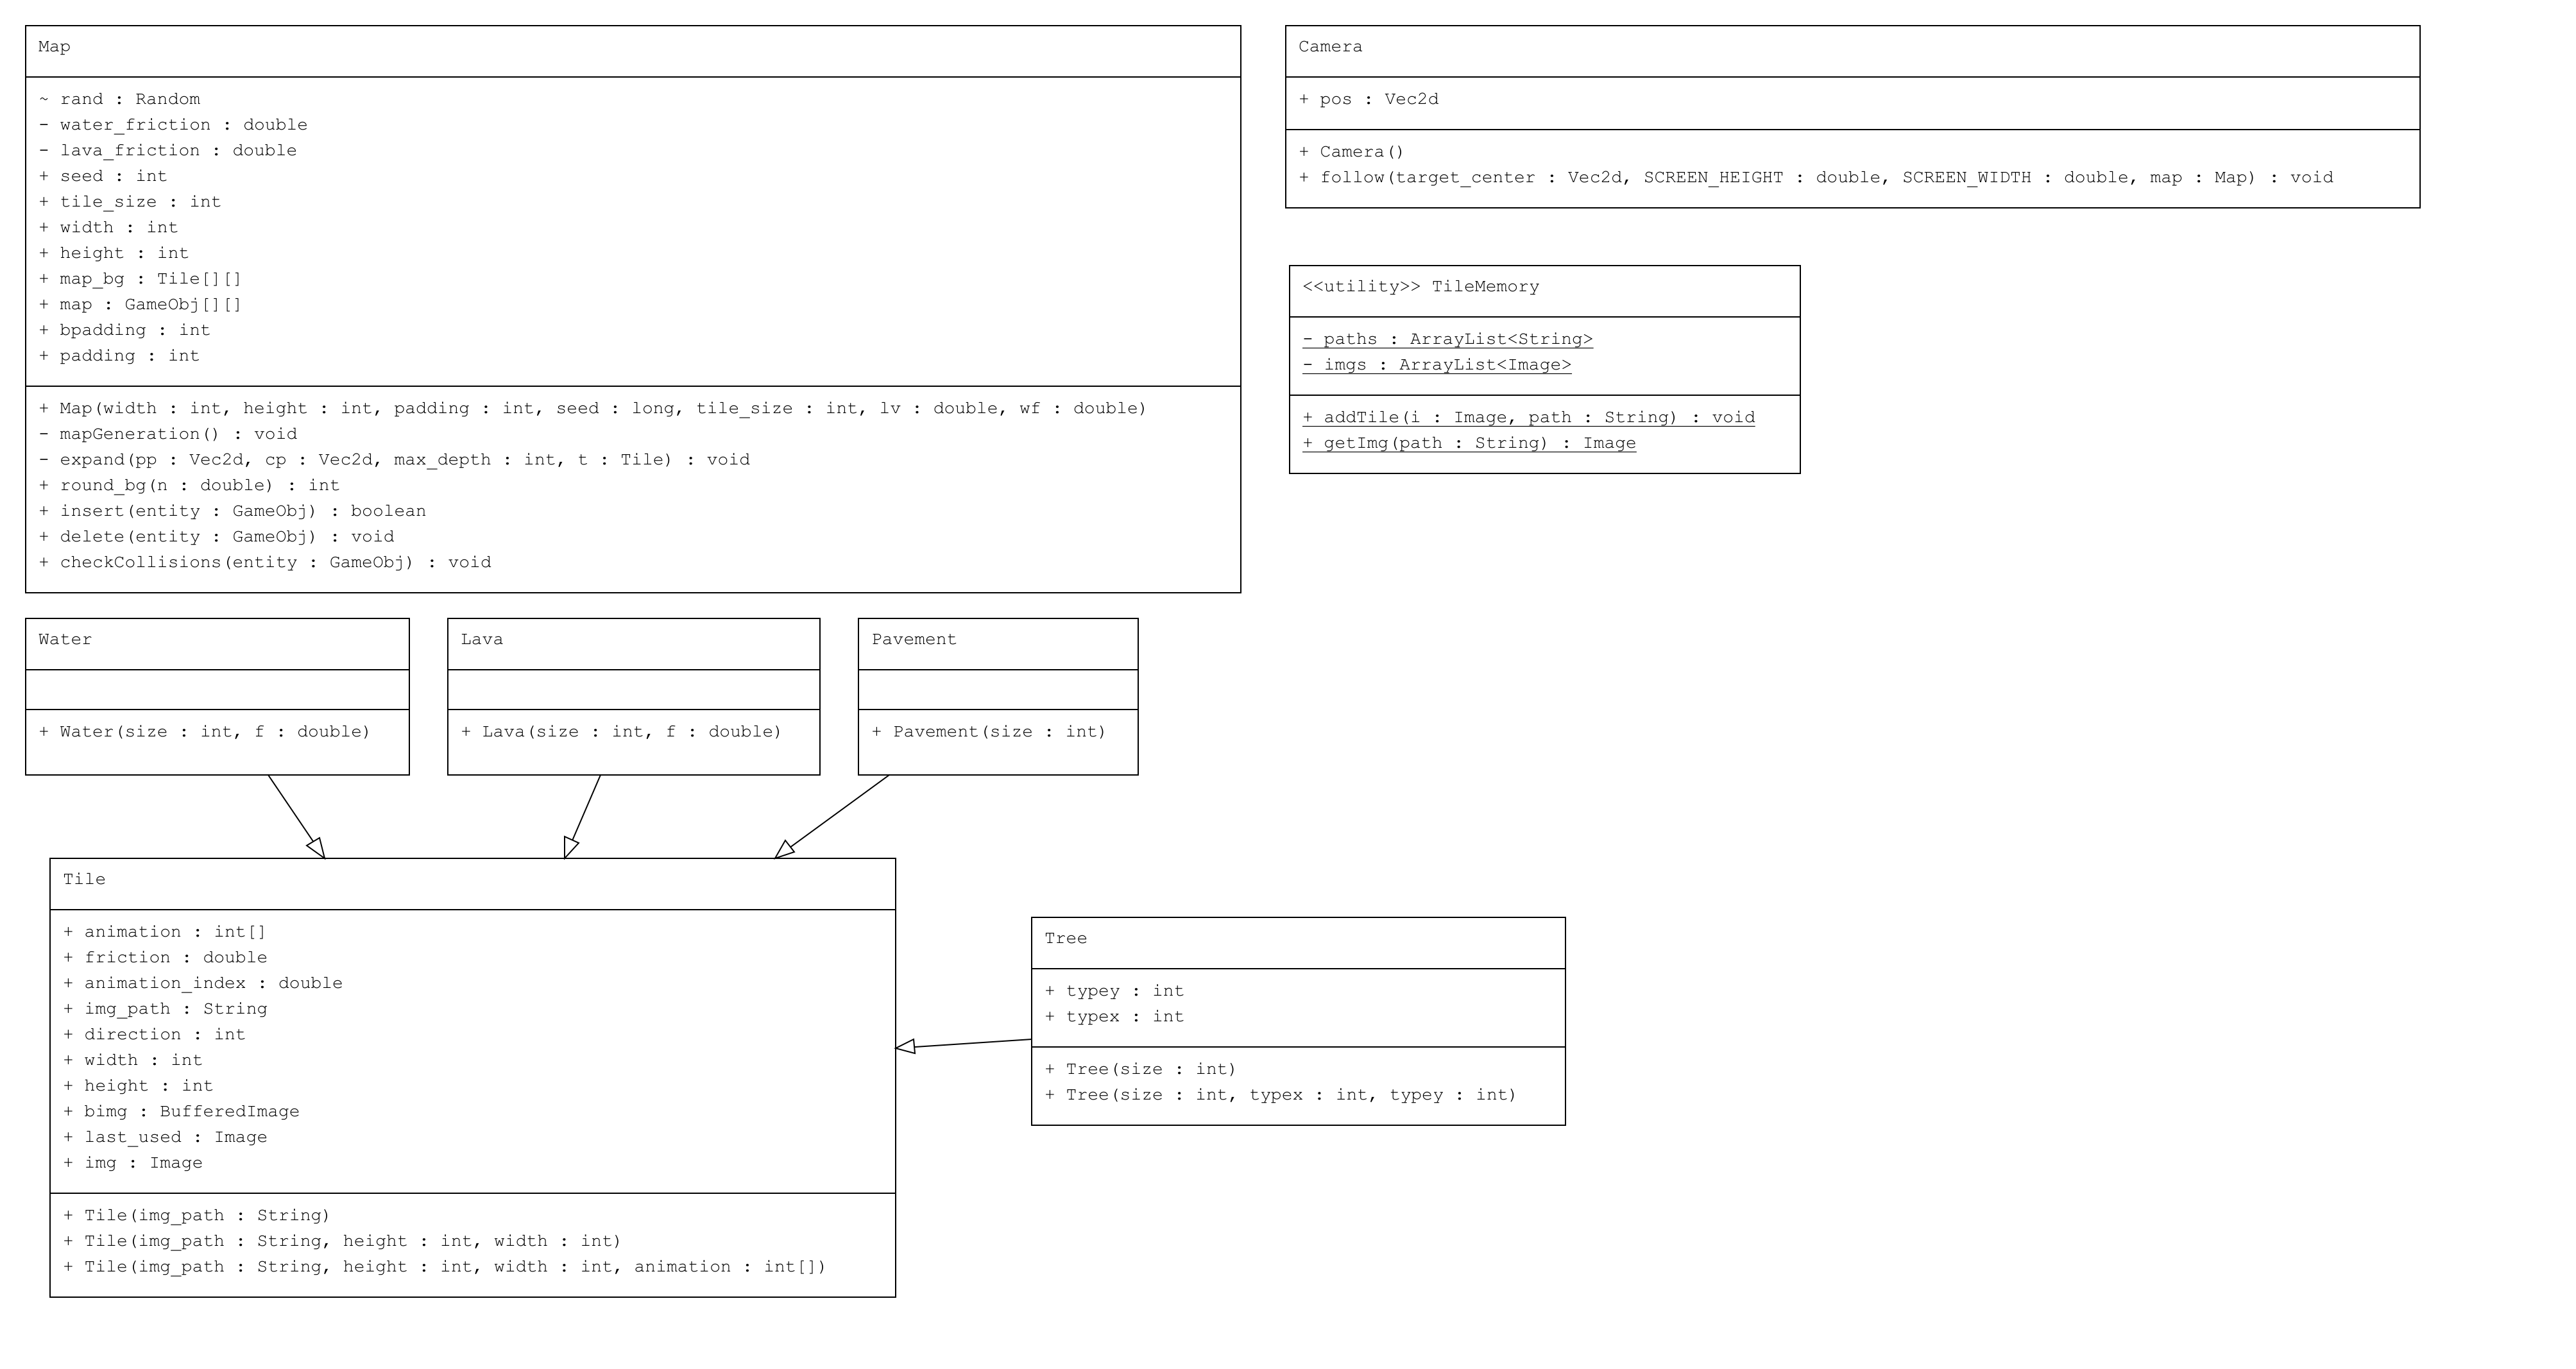
\includegraphics[width=1.2\textwidth]{LaTeX-template-PIGDM/figures/map.png}
    \caption{diagramma uml delle varie classi all'interno di map}
    \label{fig:enter-label}
\end{figure}
all'interno del pacchetto map, si trova tutta la gestione della generazione della mappa e aggiornamento posizione delle entita' e proiettili nella mappa (inoltre uso la mappa per la gestione collisioni).
Vediamo nel dettagli le classi piu' importanti:


\begin{itemize}
\item Map: la classe principale contenente le 2 mappe del gioco (per background e per posizione entita'). Vediamo i metodi piu' importanti: 
\begin{itemize}
\item mapGeneration(): genera background della mappa (con alberi lava e acqua)
\item expand(): metodo per allargare eventuali laghi o pozze di lava
\item round\_bg: utile per il cambio di variabile da map a map\_bg (non hanno dimensione uguale poiche posso ridurre le dimensioni data la dimensione fissa delle tiles del background), in modo da sapere se entita' si trova sopra lava o acqua.
\item insert(): inserisce oggetto nella mappa (inserisce solo i 4 angoli di entita', utile per il controllo collisioni)
\item checkCollisions: controlla che nell'area all'interno della posizione di un entita' non ve ne siano altre
\end{itemize}


\item Tile : questa classe sara' usata principalmente per le gestione delle skin di tutti gli oggetti. E' anche usata per la gestione delle tiles del background. Vediamo gli attributi
\begin{itemize}
\item animation: lista di numeri che indicano posizione nello sprite delle varie skin che andranno a formare un'animazione
\item direction: tiene traccia della direzione dell'oggetto al quale applichero' la skin
\item prop: JSONObject contenente tutte le impostazioni del gioco principale (come numero di nemici, dimensioni mappa ecc)
\end{itemize}

\item TileMemory: una classe di memoria utile ad evitare di caricare ogni volta le skin dalle immagini, ma si tiene in un array tutte le immagini gia' caricate
\begin{itemize}
\item addTile(): aggiunge nuova immagine nell'array
\item getImg(): restituisce immagine in memoria (se presente, altrimenti richiama addTile e poi la restituisce)

\end{itemize}
\end{itemize}
\newpage

\begin{figure}[h]
    \centering
    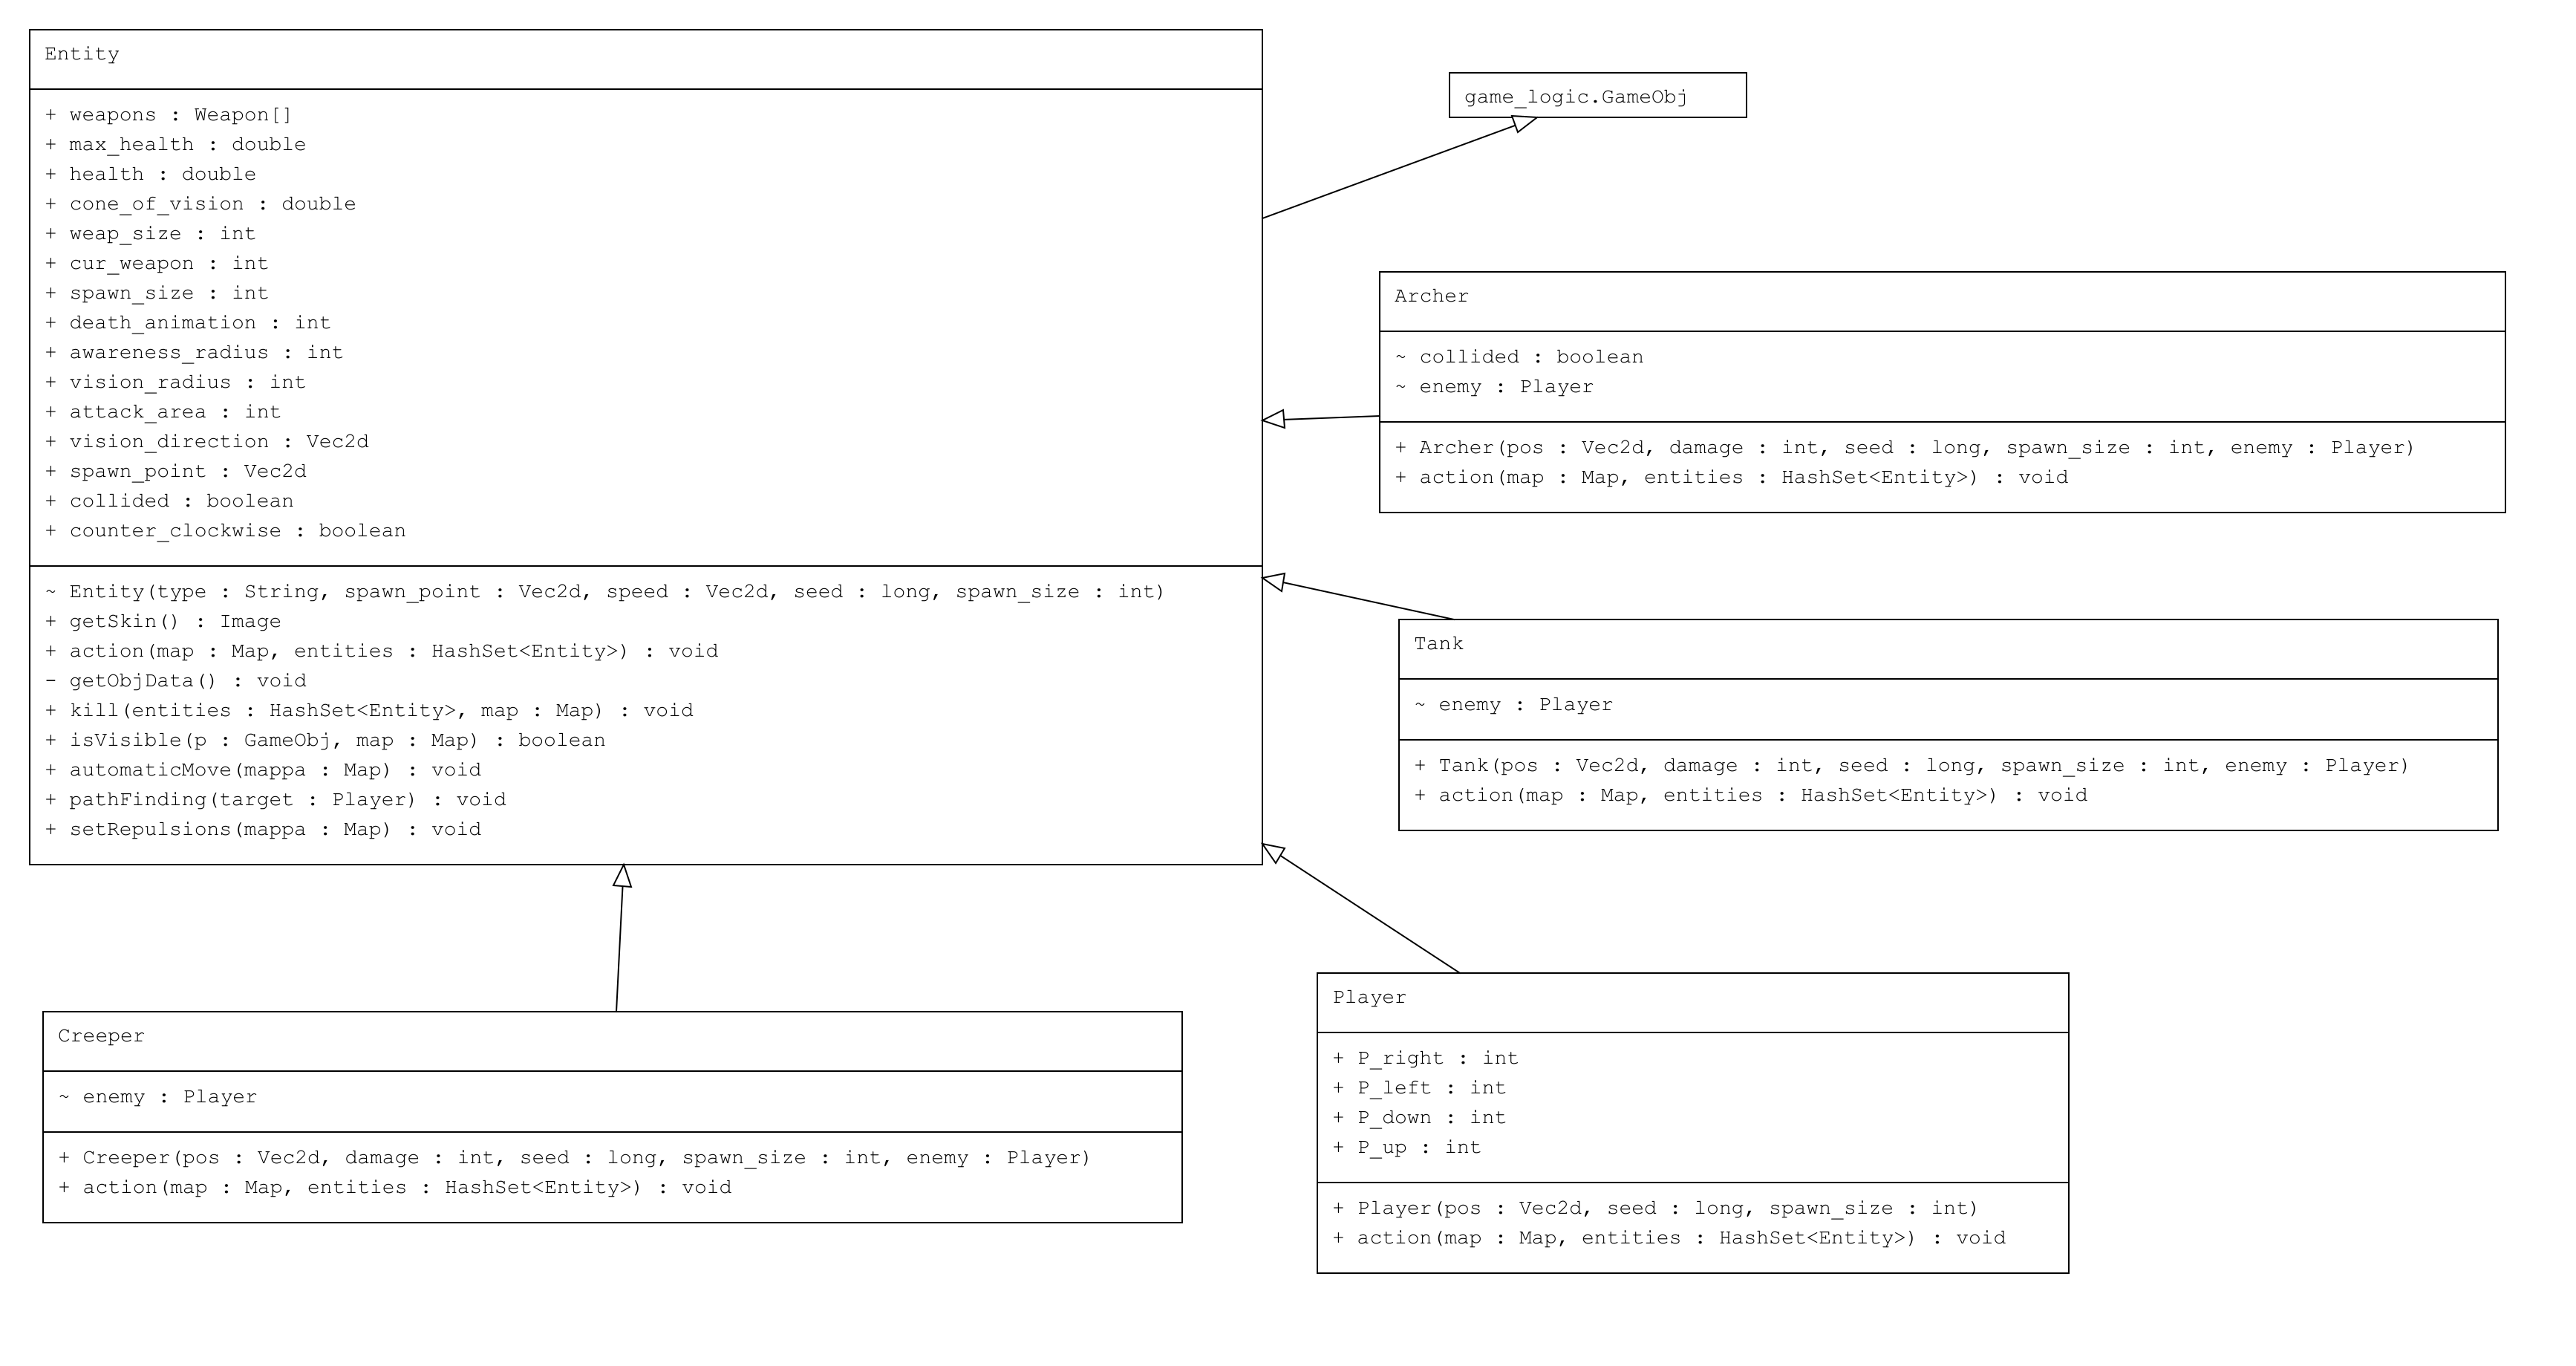
\includegraphics[width=1.2\textwidth]{LaTeX-template-PIGDM/figures/entities.png}
    \caption{diagramma uml delle varie classi all'interno di entities}
    \label{fig:enter-label}
\end{figure}
In entities vi ho inserito tutte le classi inerenti al giocatore e i vari nemici. La logica principale si trova dentro la classe Entity:

 
\begin{itemize}
\item weapons: lista di weapon di un entita' 
\item cone\_of\_vision: angolo di visione
\item awareness\_radius: raggio oltre al quale un'entita' perde di vista il giocatore
\item counter\_clockwise: direzione di rotazione dell'entita' (la aggiorno ad ogni collisione con muri o alberi)
\end{itemize}
\begin{itemize}
\item action(): invoca tutte le azioni che deve compiere l'entita' (logica di movimento e se possibile spara)
\item kill(): uccide un entita' (fa partire animazione)
\item isVisible(): controlla se entita' e' in grado di vedere il giocatore
\item automaticMove(mappa): muove in maniera automatica il nemico (movimento standard per quando non si e' in prossimita' del giocatore)
\item pathFinding(player):movimento entita' per quando si vede il nemico (si inizia l'inseguimento)
\end{itemize}


\begin{figure}[h]
    \centering
    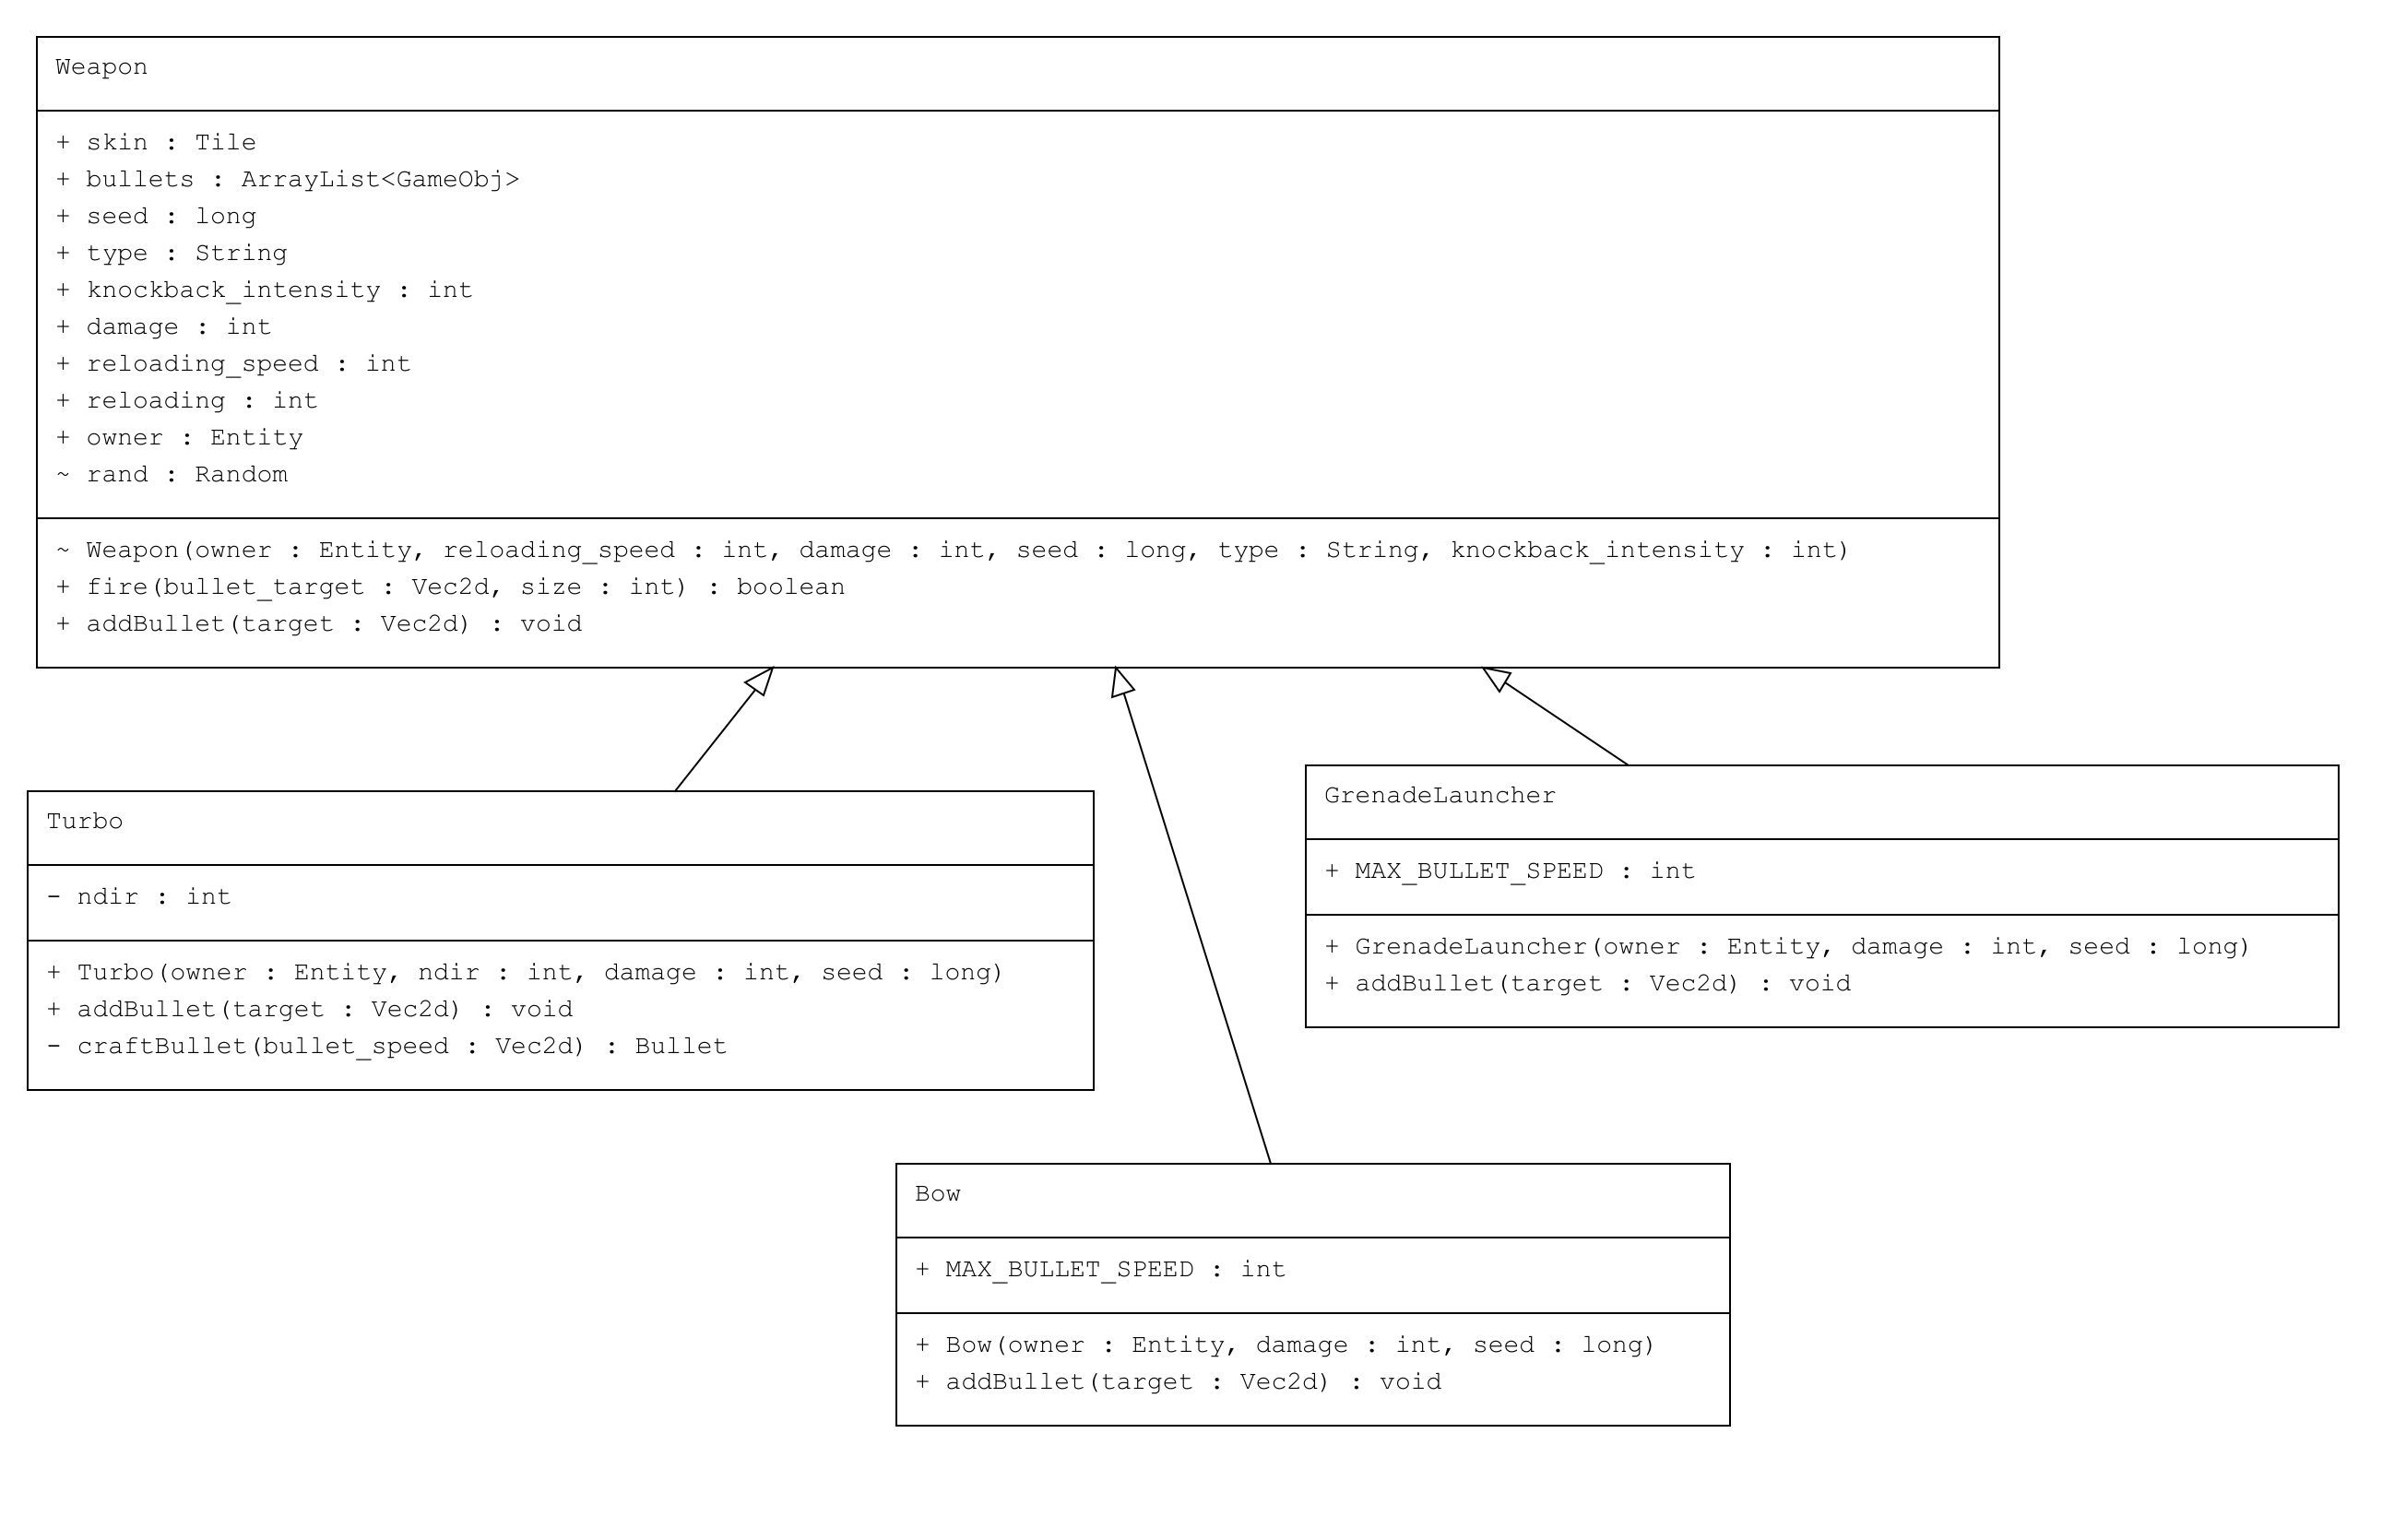
\includegraphics[width=1.2\textwidth]{LaTeX-template-PIGDM/figures/weapons.png}
    \caption{diagramma uml delle varie classi all'interno di weapons}
    \label{fig:enter-label}
\end{figure}
new pacchetto weapons ho inserito tutte le armi che si possono trovare per terra o che hanno i nemici; la struttura e' sempre orientata agli oggetti, con struttura gerarchica. Vediamo la classe principale Weapon (che verra' poi ereditata da ogni arma del gioco):
 
\begin{itemize}
\item fire(): controlla che l'entita' non debba aspettare il reloading e, se possibile, spara nella direzione passata al metodo (che verra' chiamato dal metodo action delle entita')
\item addBullet(): aggiunge proiettile alla lista proiettili da muovere nella mappa
\end{itemize}








\chapter{Problemi Riscontrati}\label{ch:prog}
Durante lo sviluppo del gioco, ho incontrato diverse sfide:
\begin{itemize}
\item Pathfinding: Trovare un algoritmo di pathfinding efficiente che permettesse ai nemici di raggiungere il giocatore in modo fluido
e naturale si è rivelato un molto difficile.Volevo riuscire ad aggiornare dinamicamente il percorso in base alla distanza dal giocatore.
\item Collisioni: La gestione delle collisioni ha richiesto una particolare attenzione. Ho dovuto implementare sistemi per prevenire che le
entità si incastrino all'interno degli oggetti o che superino i limiti della mappa.
\item Sovrapposizione delle entità: Per evitare che i nemici si ammassassero tutti nello stesso punto, ho introdotto un sistema di repulsione
basato su vettori che si intensifica man mano che le entità si avvicinano tra loro.
\end{itemize}

Soluzioni adottate:
\begin{itemize}
\item Pathfinding: Ho optato per una somma di vettori che tiene in considerazione il raggio di attacco del nemico,
in maniera da posizionarsi ad una distanza ottimale per l’attacco ed iniziare a roteare attorno al giocatore.
\item Collisioni: Ho implementato un sistema di collisioni basato su bounding box, con un meccanismo di risoluzione che prevede
lo spostamento delle entità in caso di collisione.
\item Sovrapposizione: Il sistema di repulsione basato su vettori si è rivelato efficace nel mantenere una distanza minima tra le entità.
\item Configurazione: Per facilitare la personalizzazione del gioco e renderlo più accessibile a eventuali modifiche, ho deciso di
utilizzare file JSON per memorizzare i parametri di configurazione. In questo modo, è possibile modificare vari aspetti del gioco
senza dover ricompilare il codice.
\end{itemize}
\newpage

\chapter{Conclusioni e Sviluppi futuri}\label{ch:prog}
Il progetto "ClickMania" ha rappresentato una sfida stimolante che ha permesso di approfondire le mie conoscenze nella
programmazione di videogiochi e nello sviluppo di interfacce grafiche. L'obiettivo di creare un'esperienza di gioco coinvolgente
e divertente è stato raggiunto grazie all'implementazione di meccanisiche di gioco solide e di una varieta' di personaggi e armi.

ClickMania, dati i punti nei quali ho preferito focalizzarmi sia per passione che per importanza, possiede i seguenti punti di forza:


Gameplay fluido: Il sistema di movimento dei personaggi, la gestione delle collisioni e la decisione di animare e aggiornare solo
le entita' visibili, garantiscono un'esperienza di gioco scorrevole e reattiva.\\
Varietà di gioco: La presenza di diversi tipi di nemici e armi contribuisce a rendere il gameplay dinamico e a evitare la ripetitività.\\
Generazione procedurale: La generazione procedurale dei livelli aumenta significativamente la rigiocabilità,
offrendo al giocatore un'esperienza sempre diversa.\\\\

Tuttavia, sono emerse anche alcune limitazioni:

Grafica: La grafica, pur essendo funzionale, potrebbe essere migliorata per rendere il gioco visivamente più accattivante.\\
Suono: L'assenza di effetti sonori e di una colonna sonora dedicata limita l'immersività dell'esperienza di gioco.\\
Path finding piu' intelligente: il pathfinding dei nemici, sebbene funzionale, potrebbe essere ulteriormente sviluppato
per rendere i combattimenti più sfidanti e strategici.\\

\section{Sviluppi futuri}\label{ch:arch}
Sulla base delle considerazioni precedenti, si prospettano le seguenti linee di sviluppo futuro:

Miglioramento della grafica:
Introduzione di effetti particellari, animazioni dei personaggi durante l'attacco e anche quando sono immobili, in maniera 
da arricchire le animazioni e le esplosioni.\\

Implementazione di un sistema di camera top down piu' dinamico per creare atmosfere più suggestive e dare piu' un feel 
di tridimensionalita' al gioco, pur essendo 2D.\\\\

Espansione del gameplay:
Aggiunta di nuovi tipi di nemici con abilità speciali e pattern di attacco più complessi.
Introduzione di boss fight per aumentare la sfida e offrire momenti di climax.\\

Generazione di mappe piu' complesse e realistiche (con biomi piu' coerenti e punti di spawn di nemici riconoscibili)\\\\


Personalizzazione:
Permettere al giocatore di personalizzare l'aspetto del proprio personaggio e delle armi.\\

Introduzione di un editor di livelli per consentire agli utenti di creare i propri livelli e condividerli con la community.\\

Inoltre, si potrebbe considerare l'integrazione di un sistema di progressione più articolato, con l'introduzione di 
abilità sbloccabili e di un sistema di livellamento.

\end{document}